% !TEX root =  main.tex

\section{The DARC Toolbox}
\label{sec:design:darc}

\begin{figure}[t]
	\centering
	\begin{subfigure}[b]{0.49\textwidth}
		\centering
		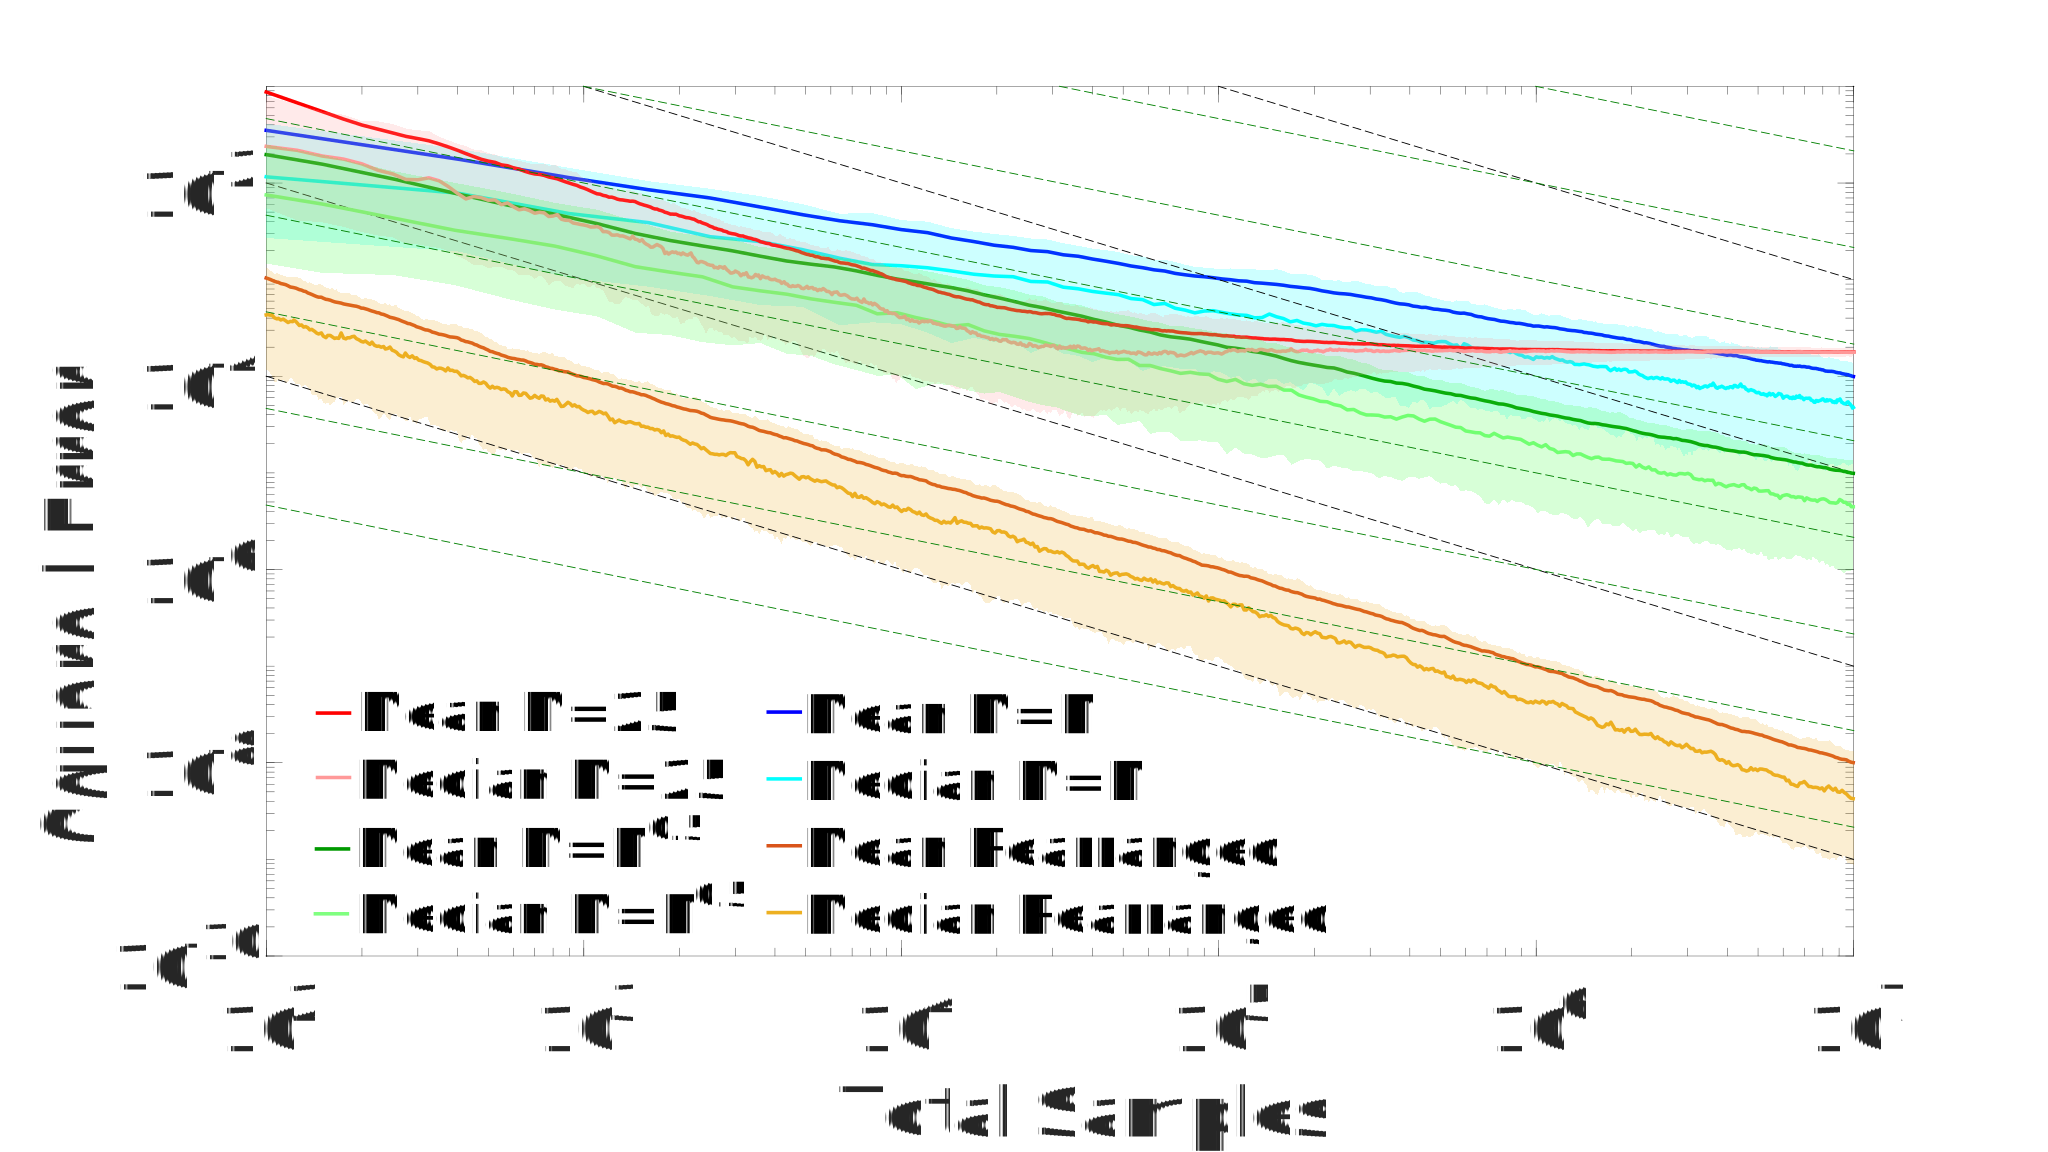
\includegraphics[width=0.99\textwidth,trim={1.5cm 0 3.5cm 0},clip]{exp_conv2}
		\caption{Convergence of BED\label{fig:exp-conv}}
	\end{subfigure}
		\begin{subfigure}[b]{0.49\textwidth}
			\centering
			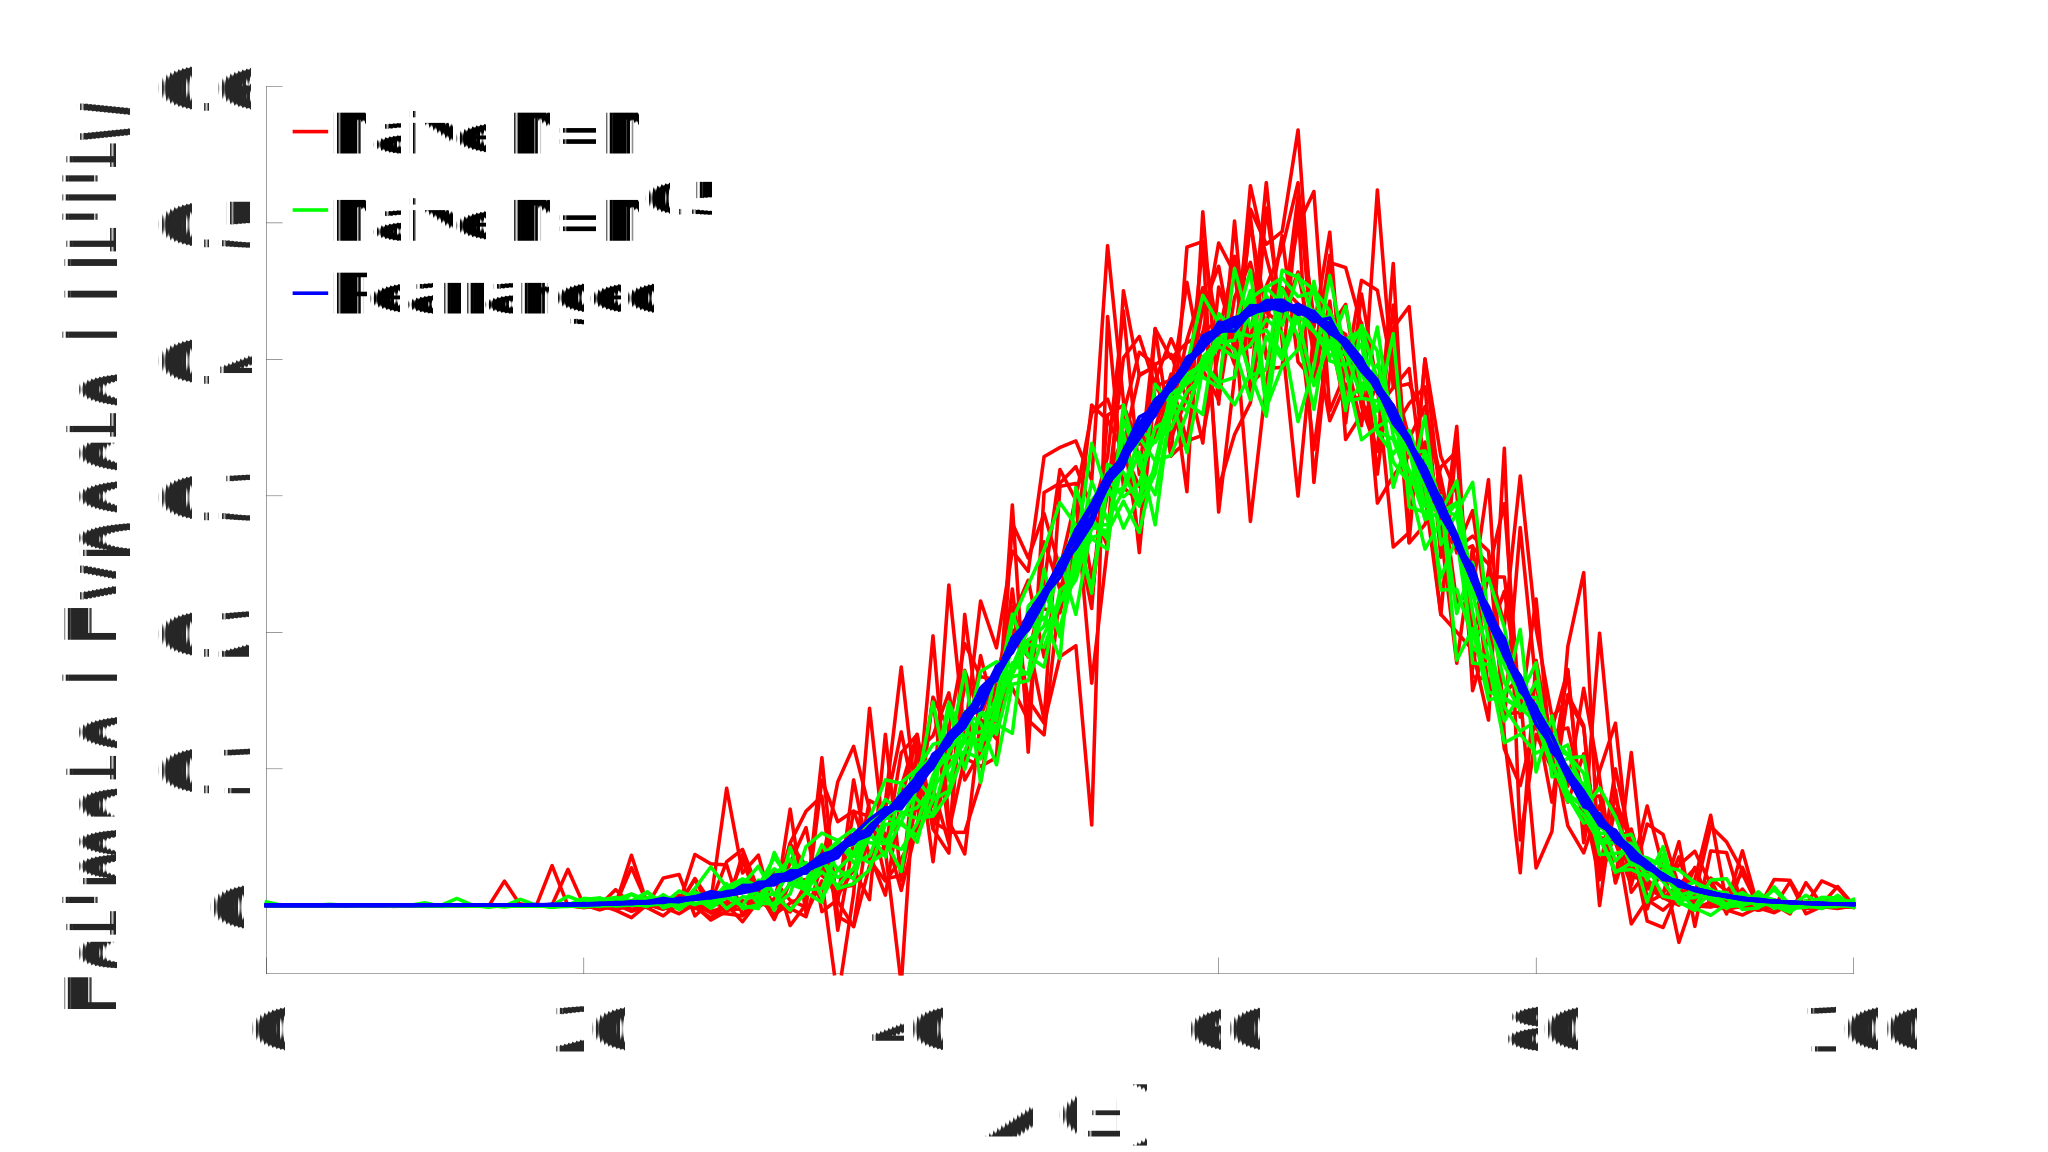
\includegraphics[width=0.99\textwidth,trim={1.5cm 0 3.5cm 0},clip]{dscan_2}
			\caption{Estimated expected utilities \label{fig:exp-d-scan}}
		\end{subfigure}
	\caption{(Left) convergence of both NMC and our reformulated
		estimator~\eqref{eq:u_bar_MC} for the BED problem.
		A ground truth estimate was calculated using a single run of the reformulated
		estimator with $10^{10}$ samples.
		Results are averaged over 1000 independent runs, while shaded regions give the 25\%-75\% quantiles. We
		see that the theoretical convergence rates are observed in all cases,
		with the advantages of the reformulated estimator particularly pronounced.
		(Right) estimated expected utilities $\bar{U}(d)$for 
		different values of one of the design parameters $A \in \{1,2,\dots,100\}$ given a fixed total
		sample budget of $T=10^4$.  Here the lines correspond to 10 independent runs, showing
		that the variance of \eqref{eq:exp-des-nmc} is far higher than \eqref{eq:u_bar_MC}.
		}
\end{figure}

We now demonstrate that the theoretical improvements provided by our estimator carry over
to practical gains, using as a case study our recent work~\cite{vincent2017darc}, in which we
construct a package for adaptive psychology experiments investigating the effects of
delays and risks on the subjective value people give to money. Our so-called DARC (Delay And Risky Choice)
toolbox\footnote{Available at \url{github.com/drbenvincent/discounting-experiment-toolbox}} allows users 
to encode their own (or use one of the provided) models for human \emph{discounting} behavior,
whereby psychologists want to learn how delays and uncertainties affect the subjective value people place
on rewards or costs. Given a model, the toolbox automates in an online fashion 
both the inference of the model parameters and the sequential adaptation of the experiment itself through
choosing the questions the participant is asked.  It therefore automates the full run-time experimental 
pipeline  by using the responses from previous questions to perform inference 
and update the internal representation
of the participant and then using information to ask the most informative questions for a particular
participant as per the BED equations.  Our reformulated estimator is one of a number of key technical
innovations that are essential in allowing this to be done sufficiently efficiently to permit
real-time usage required for deployment with real participants.  It is beyond the scope of our current
work to explain how this is done 

More specifically how delays or uncertainties in rewards 


To demonstrate the improvements introduced by our estimator
we consider a model used in psychology experiments for delay discounting introduced by 
\cite{vincent2016hierarchical} and later adapted by \cite{vincent2017darc}.  Our experiment 
comprises of asking questions of the form 
\emph{``Would you prefer $\pounds A$ now, or $\pounds B$ in $D$ days?''} and we wish 
to choose the question  variables $d = \{A,B,D\}$ in the manner that will give the most 
incisive questions.  The target participant is presumed to have parameters $\theta=\{k,\alpha\}$ 
and the following response model
\begin{equation}
y \sim \mathrm{Bernoulli} \left(0.01 + 0.98 \cdot \Phi\left(\frac{1}{\alpha} \left(\frac{B}{1+e^k D}-A\right)\right)\right)
\end{equation}
where $y=1$ indicates choosing the delayed response and $\Phi$ represents the 
cumulative normal distribution.  As more questions are asked, the distribution 
over the parameters $\theta$ is updated, such
that the most optimal question to ask at a particular time depends on the previous questions
and responses.  For the sake of brevity, when comparing the performance 
of~\eqref{eq:exp-des-nmc} and~\eqref{eq:u_bar_MC} we will neglect the problem 
of how best to optimize the design, and consider
only the problem of evaluating $\bar{U}(d)$.  We will further consider the case 
where $B=100$ and $D = 50$ are fixed and we are only choosing the delayed value $A$.
Our prior distributions on the parameters are given by $k \sim \mathcal{N}(-4.5,0.5^2)$
and $\alpha \sim \Gamma(2,2)$.
We first consider convergence in the estimate of $\bar{U}(d)$ for the case $A=70$ for our suggested method~\eqref{eq:u_bar_MC} and the na\"{i}ve solution~\eqref{eq:exp-des-nmc}, the results of which are shown in Figure~2a in the main paper. 
Here we see that the convergence rates of the two methods are both as expected and that our suggested method offers significant empirical performance improvements.  

We next consider setting a total sample budget $T=10^4$ and look at the variation in the estimated values of $\bar{U}(d)$ for different values of $A$ for the two methods as shown in Figure~\ref{fig:exp-d-scan}.
This shows that the improvement in MSE leads to clearly visible improvements in the characterization of $\bar{U}(d)$ that
will translate to improvements in seeking the optimum.